% !TeX encoding = UTF-8
% !TeX spellcheck = en_US
% !TeX root = report1.tex

\section{Variational}
 Now we focus on using the integration to solve the problem established in the introduction.
 Using the Monte Carlo integration we focused on three different problems, the harmonic oscillator,
 hydrogen atom and helium atom.

\subsection{Harmonic Oscillator}
The Hamiltonian of the harmonic oscillator is
\begin{align*}
  \hat{H} = \frac{-1}{2}\frac{\partial^2}{ \partial x^2} + \frac{1}{2} x^2.
\end{align*}
Where we choose the trial wave function as
  \begin{align*}
    \Psi_T = e^{-\alpha x^2}.
  \end{align*}
From this we can derive tha local energy
  \begin{align*}
    E_L = \alpha + x^2(\frac{1}{2} - 2\alpha^2).
  \end{align*}
 	
  Notice that based on the local energy we can already determine that $\alpha = \frac{1}{2}$ gives us the ground state ($E_L = E_0 = \frac{1}{2}$), because in that case the variance of the local energy is equal to zero. It is nonetheless a good test for our algorithm to see if we can find the expected value of $E_0 = \frac{1}{2}$ using Monte Carlo integration.  \\
  
We apply the stratified adaptive integration scheme as defined in section 3 and use Newton's method on the derivative $\frac{dE}{d\alpha} = 2 (<E_L \frac{d \ln \Psi_T}{d \alpha}> - E<\frac{d \ln \Psi_T}{d \alpha}>)$. This method works because our the exact solution is within the family of trial functions, see [reference to book]. In 100 steps we reached an energy of $E_{MC} = 0.50000000163$ at $\alpha = 0.500001076455$.  See [awesome graph that Ren\'e will give us] where we show the value of the energy as a function of iteration number and as a function of $\alpha$. 

[INSERT GRAPH HERE. CAPTION: Energy as a function of iteration number (left) and alpha (middle), and alpha again but on a log-scale (right). Notice that after there is a limited accuracy we can achieve, due to the damping factor being of finite nature.  
  

\subsection{Hydrogen Atom}
We will now consider the Hydrogen atom, where the Hamiltonian is
\begin{align}
  \hat{H} = \frac{-1}{2}\nabla^2 - \frac{1}{r}.
\end{align}

We choose the trial wave function as
  \begin{align}
    \Psi_T = e^{-\alpha r}.
  \end{align}
This leads the a local energy
  \begin{align}
    E_L(r) = - \frac{1}{r} - \frac{1}{2}\alpha(\alpha - \frac{2}{r})
  \end{align}

Here, too, we notice that from inspection it is clear that $\alpha = 1$ yields the ground state energy of $E_L = E_0 = -\frac{1}{2}$, because there $Var(E_L) = 0$.




\subsection{Helium Atom}
Finally we consider the Hamiltonian for the helium atom,
\begin{align}
  \hat{H} = -\frac{1}{2}(\nabla_{r_1}^2 + \nabla_{r_3}^2 + 2\nabla_{r_1}\cdot \nabla_{r_2}) - \frac{1}{r}.
\end{align}
Where will we use the trial function
  \begin{align}
    \Psi_T (\textbf{r}_1,\textbf{r}_2) = e^{2r_1}e^{2r_2}e^{\frac{r_{12}}{2(1+\alpha r_{12}}}
  \end{align}

where $r_{12} = |\textbf{r}_1 - \textbf{r}_2 |$. This trial function is applied to the following Hamiltonian:


This leads a 'beautiful' equation for the local energy:
  \begin{align}
    E_L(\textbf{r}_1,\textbf{r}_2) = -4  + (\hat{\textbf{r}}_1 - \hat{\textbf{r}}_2) \cdot (\textbf{r}_1 - \textbf{r}_2) \frac{1}{r_{12}(1+\alpha r_{12})^2} -  \frac{1}{r_{12}(1+\alpha r_{12})^3} - \frac{1}{r_{12}(4(1+\alpha r_{12}))^4} + \frac{1}{r_{1,2}}   \end{align}
  
This, too, we solved with using the stratified adaptive integration method, and changing $\alpha$ like we did at the Harmonic Oscillator and the Helium atom. Using two different starting values $\alpha_0$ we convergence to the same values for $\alpha$ and $E_{MC}$, see figure [awesome graph]. The values we find the energy after just 50 iterations are $E_{\alpha_0 = 0.5} =  $ and $E_{\alpha_0 = 0.5} =  $, which compare well with the optimum value achieved by this method of $-2.8781 \pm 0.0005$, the Hartree-Fock value of $-2.8617$, the DFT value of $-2.83$ and the exact value of $-2.9307$ (see [reference to book]). 

\begin{figure}
  \begin{center}
  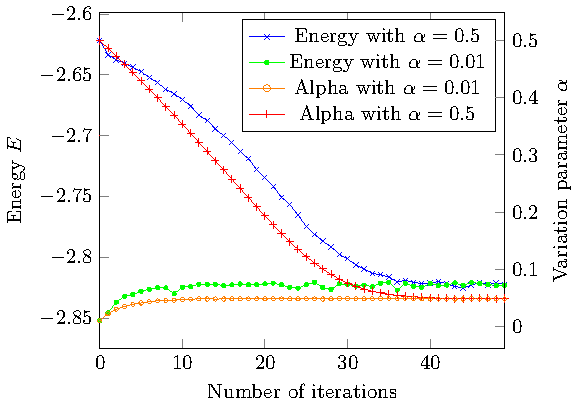
\includegraphics[scale=1 ]{graphs/he-e-alpha-iterations.pdf}
  \caption{Calculated $E$ as a function of $\alpha$ using two different starting values for$\alpha_0$. Notice that $\alpha$ converges monotonically (increasing or decreasing) while this is not necessarily true for the energy due to the integration not being exact. Nonetheless, a very accurate result can be found: $E_{\alpha_0 = 0.5} =  $ and $E_{\alpha_0 = 0.5} =  $}
  \label{fig:He_it}
  \end{center}
\end{figure}
 
